\documentclass[border=1pt]{standalone}
\usepackage{tikz}
\usetikzlibrary{lindenmayersystems}

\setcounter{errorcontextlines}{999}
\begin{document}
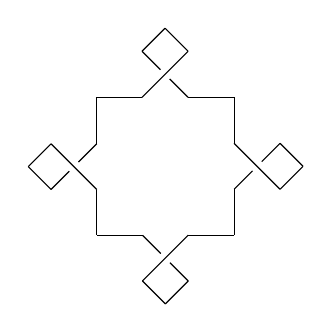
\begin{tikzpicture}[scale=.05]
  \pgfmathsetmacro{\midfac}{1.4142135623730951}

  \pgfmathsetmacro{\halfmidfac}{.5*\midfac}
  \pgfmathsetmacro{\invhalfmidfac}{2.82842712474619}

  \pgfmathsetmacro{\posa}{.4*\midfac}
  \pgfmathsetmacro{\posb}{.6*\midfac}
  % \pgfmathsetmacro{\posc}{\midfac}

  \pgfdeclarelindenmayersystem{kochknot}{
    % Scale
    \symbol{S}{\pgflsystemstep=.3333333333333333\pgflsystemstep}

    % Restore
    \symbol{R}{\pgflsystemstep=3\pgflsystemstep}

    % Scale 2
    \symbol{T}{\pgflsystemstep=\halfmidfac\pgflsystemstep}

    % Restore 2
    \symbol{U}{\pgflsystemstep=\midfac\pgflsystemstep}

    \symbol{A}{
      \draw (0,0) -- (\pgflsystemstep, 0);
      \tikzset{xshift=\pgflsystemstep}
    }

    \symbol{a}{
      \draw (0,0) -- (\pgflsystemstep, 0);
      \tikzset{xshift=\pgflsystemstep}
    }

    % Ascending ramp thing
    \symbol{B}{
      \draw (0,0) -- (\midfac\pgflsystemstep, 0);
      \tikzset{xshift=\midfac\pgflsystemstep}
    }

    % Break in strand
    \symbol{C}{
      \draw (0,0) -- (\posa\pgflsystemstep, 0);
      \draw (\posb\pgflsystemstep, 0) -- (\midfac\pgflsystemstep, 0);
      \tikzset{xshift=\midfac\pgflsystemstep}
    }

    \rule{A -> SA+B++Ta++aU++C+AR}
    \rule{a -> Sa-B--TA--AU--C-aR}
  }


  \draw l-system [l-system={kochknot, axiom=A--A--A--A, order=1, angle=45, step=1000}];
\end{tikzpicture}
\end{document}
